% @HEADER
% ***********************************************************************
%
%            Trilinos: An Object-Oriented Solver Framework
%                 Copyright (2001) Sandia Corporation
%
% Under terms of Contract DE-AC04-94AL85000, there is a non-exclusive
% license for use of this work by or on behalf of the U.S. Government.
%
% This library is free software; you can redistribute it and/or modify
% it under the terms of the GNU Lesser General Public License as
% published by the Free Software Foundation; either version 2.1 of the
% License, or (at your option) any later version.
%
% This library is distributed in the hope that it will be useful, but
% WITHOUT ANY WARRANTY; without even the implied warranty of
% MERCHANTABILITY or FITNESS FOR A PARTICULAR PURPOSE.  See the GNU
% Lesser General Public License for more details.
%
% You should have received a copy of the GNU Lesser General Public
% License along with this library; if not, write to the Free Software
% Foundation, Inc., 59 Temple Place, Suite 330, Boston, MA 02111-1307
% USA
% Questions? Contact Michael A. Heroux (maherou@sandia.gov)
%
% ***********************************************************************
% @HEADER

\documentclass[11pt,relax]{SANDreport}
\usepackage{graphicx}
\usepackage{amsmath,amsfonts,amsthm}
\usepackage{amssymb}
\usepackage{enumerate}
\usepackage{rotating}


\usepackage{times}

\def\choicebox#1#2{\noindent$\hphantom{th}$\parbox[t]{1.8in}{\sf
#1}\parbox[t]{4.5in}{#2}\\[0.8em]}

\author{Sala, Phenow, Hu, Tuminaro}

\title{MatrixPortal: a Web-based Tools for Performance Analysis of Sparse Linear
Algebra Libraries}
\SANDnum{SAND2006-XXXX}
\SANDauthor{Sala, Phenow, Hu, Tuminaro}

\SANDprintDate{July 2006}
\SANDreleaseType{Unlimited Release}

\newcommand{\Trilinos}{Trilinos}
\newcommand{\TrilinosTM}{Trilinos \copyright}
\newcommand{\trilinos}{{\sc Trilinos}}
\newcommand{\ifpack}{{\sc Ifpack}}
\newcommand{\aztecoo}{{\sc AztecOO}}
\newcommand{\amesos}{{\sc Amesos}}
\newcommand{\epetra}{{\sc Epetra}}
\newcommand{\ml}{{\sc ML}}
\newcommand{\mb}[1]{{\mathbf {#1} }}
\newcommand{\teuchos}{{\sc Teuchos}}
\newcommand{\triutils}{{\sc Triutils}}
\newcommand{\metis}{{\sc METIS}}

\newcommand{\ie}{i.e., }
\newtheorem{assumption}{Assumption}[section]
\newtheorem{lemma}{Lemma}[section]
\newtheorem{proposition}{Proposition}[section]
\newtheorem{corollary}{Corollary}[section]
\newtheorem{theorem}{Theorem}[section]
\newtheorem{algorithm}{Algorithm}[section]
\newtheorem{definition}{Definition}[section]
\newtheorem{property}{Property}[section]

\newtheorem{remark}{Remark}
\newtheorem{problem}{Problem}

\def\choicebox#1#2{\noindent$\hphantom{th}$\parbox[t]{3.0in}{\sf
#1}\parbox[t]{3.35in}{#2}\\[0.8em]}

\begin{document}

\maketitle

\begin{abstract}
Mathematical software is a subfield of computer science
characterized by a mixture of algorithms and numerics. Although elegant
theoretical results have been proved for a variety of problems, there is
typically no theory that can help to individuate the best algorithm for a
given problem or a set of problems. Often, proofs involve constants that
cannot, or is not convenient to be measured. Therefore, practical experience
is very often the last resort, and sometimes the only one for certain classes
of problems. Finding the best optimal algorithm in a given parameter space is
a tedious, error prone and long activity, which involves change of parameters,
and recording of results. As such, this activity can greatly benefit for
automation.  What we aim to present in this document is a set of tools that
can help to  evaluate the performances of scientific software, and in
particular of linear algebra libraries for high-performance computing. We
present the design and implementation of a  web interface that offers
a widely accessible, homogeneous
and easy-to-use graphical interface to a suite of linear algebra solvers.
This user-friendly interface promotes testing and
experimenting with a variety of state-of-the-art linear algebra libraries for
distributed sparse matrices.
\end{abstract}

\clearpage

\SANDmain

\tableofcontents

\clearpage
\newpage


% ------------------------------------------------------------------------- %
\section{Introduction}
% ------------------------------------------------------------------------- %

Performance analysis if a key step in the design of any new
software library, in order to provide the highest performance at the lowest
cost. 

There are several motivations for measuring
the performance of linear algebra libraries, including:
\begin{itemize}
\item {\sl Validation of the library itself}.
The only way to demonstrate that the library meets its
performance goals for a given application is to measure performance under realistic
conditions.
\item {\sl Validation of an application}. The best way to validate a
performance model is to compare the model predictions to measured
performance, using well-tested and reliable solvers.
\item {\sl Support.} Developers often have to respond to value complaints of
poor performances. Offering an easy tool for testing can alleviate the
pressure on developers, and help users to fix the problem.
\item {\sl Fine tuning}.
\item {\sl Teaching}.
\item {\sl Library evaluation}.
Linear algebra libraries for distributed parallel computing require an
intensive effort to compile and optimize. Often, however, these libraries are
used to perform basic performance evaluations on standard tests cases. Making
it available all these functionalities through the
web, without installing any single component of the library on the user's
machine, can favor the use of the library.
\end{itemize}

Our system is structured as follows:
\begin{itemize}
\item select the problem of interests;
\item specify the solution parameters;
\item specify the evaluation metrics;
\item solve the problems and perform the evaluation;
\item analyze and present data.
\end{itemize}

Properly selected and
measured data can be very useful for future performance analysis.
One use is estimating the performance of customer applications on
a product, based on fundamental operations. For example,
measurements of the time need to scan, update or create database
records could be used to predict performance of specific queries
against the database. The same data is useful for modeling new
products.

\smallskip

\begin{figure}
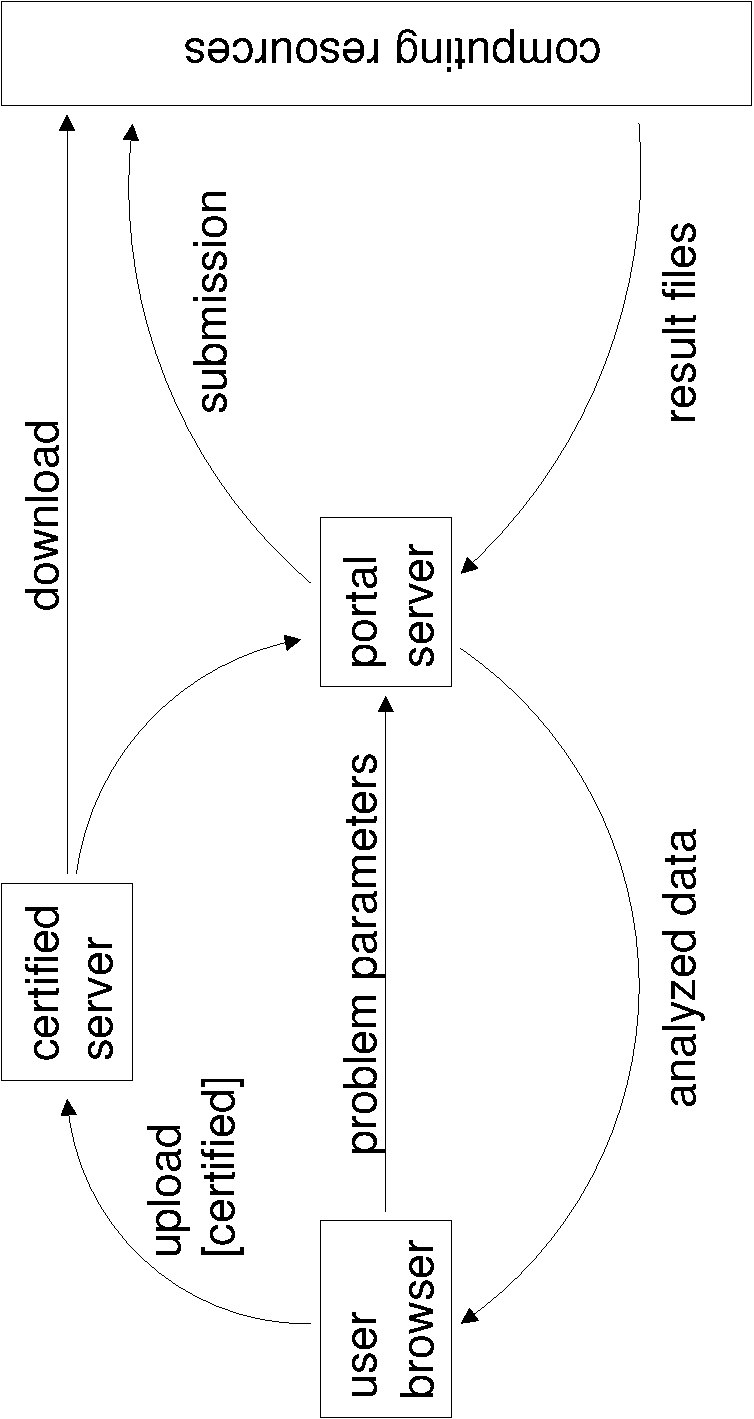
\includegraphics[width=7cm,angle=-90]{portal_design}
\caption{Design}
\label{fig:design}
\end{figure}

\begin{figure}
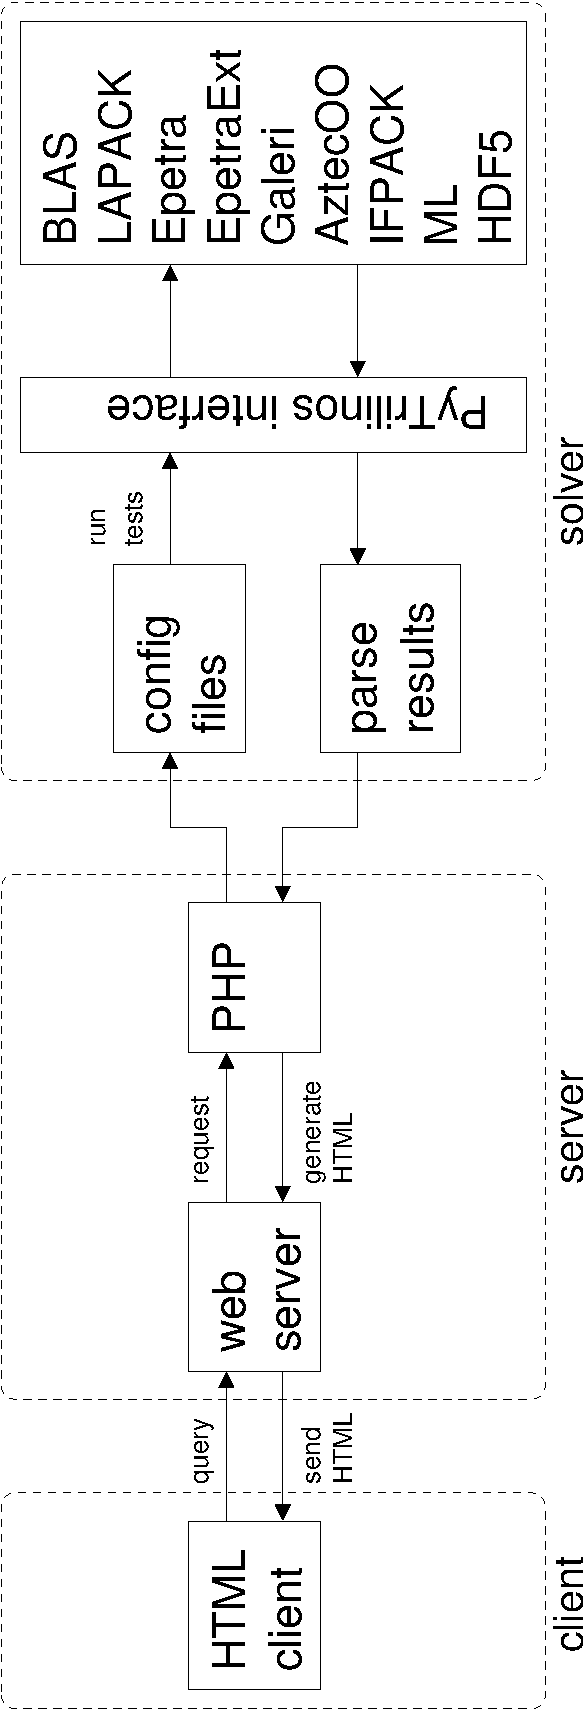
\includegraphics[height=18cm,angle=-90]{diagram}
\caption{Implementation diagram.}
\label{fig:design}
\end{figure}

An overview of the structure is reported in Figure~\ref{fig:design}.
Our portal is organized in a three-layer structure. While the user's interface
resides on the client, the middle layer and the solver layer can be located in
the same machine, or as two separate services. In the first case, we have a
Client-Server service, in the latter a Client-Server-Solver. The solver layer
could be located on the Grid; in this case we call the structure
Client-Server-Grid.

\medskip

This report is organized as follows.

% ------------------------------------------------------------------------- %
\section{Brief Overview of Performance Analysis}
% ------------------------------------------------------------------------- %

We now give a basic overview of the terminology used in performance analysis.
For an overview on the subject, we refer to~\cite{jain91art}.

Performance analysis of mathematical software can be divided into two classes:
theoretical (or analytical) modeling and performance measurement (benchmarking).
All analytic techniques require the
construction of a model, an abstract representation of the real system. 
Performance measurement does not
use models but instead relies on direct observation of the system of interest,
or a similar system.
A proper performance analysis required that the effect of each factor can be
isolated from those of others so that meaningful statements can be made about
different levels of the factors.

{\sl response variable} is the outcome of the experiment. Generally, this is
the measured performance of the system. 
{\sl Factors:} each variable that affects the response variable and has
several alternatives. Usually divided into primary and secondary factors.

The values that a factor can assume are called {\sl levels}. 

The entity that is used for the experiment is called an {\sl experimental
  unit}.

\smallskip

The term {\sl test workload} denotes any workload used in performance studies.
A test workload can be real or synthetic. A real workload is one observed on a
system being used for normal operations. A synthetic workload, whose
characteristics are similar to those of the real workload, and can be applie
repeatedly in a controlled manner, is developed and used for studies. The main
reason for using a synthetic workload is that it is a representation of a
model of a real world. As such, a theoretical estimate can sometimes be
available, and can be used to validate the system. Besudes, synthetic worload
can be easily modified and generated, and ported to different systems. Real
workload might also contain sensitive data.

A {\sl monitor} is a tool used to abserve the activity of a system. It is the key
step in performance measurement. 

% ------------------------------------------------------------------------- %
\section{Design Overview}
% ------------------------------------------------------------------------- %

% ------------------------------------------------------------------------- %
\subsection{User Interface Requirements}
% ------------------------------------------------------------------------- %

We designed our user interface as a Web service.
A Web service is a piece of functionality, exposed through a web interface.
Any authorized client on the internet can use this functionality. The server
can either send the result as a web page (HTML format), or send the response
both through an XML message or a e-mail. There are several advantages in using
web services to perform computations:
\begin{itemize}
\item XML and HTML are industry standard;
\item No special-purpose hardware is required for running web services;
\item Since the services reside only on the web server(s), the client software
does not need to be updates every time the web service is modified. Changes to
the interfaces simply need a "reload" procedure;
\item The web service code never leaves the server, so property code is
protected;
\item Web services can be accessed from everywhere; no special
purpose interface is necessary.
\end{itemize}
However, in the context of linear algebra, there are some limitations to the
utilization of web services:
\begin{itemize}
\item the data and results can be quite large, and there is no standard way to
communicate these objects;
\item intermediate results cannot be shown.
\end{itemize}

Web standards have been conceived to support interoperability, i.e.,
    independence of the transport protocols, programming languages,
    programming models, and system software. The main actors in a Web service
    architecture are requestors and providers. Requestors access services from
    providers. The added-value for the requestors will be improved by
    customized services.

Connected to the previous point is the presentation of the results. The final
goal of our analysis is to provide insight of the problem, and guidelines to
help the decision-making processing the user's application. Conveying the
results in a clear and understandable way is a major objective of our work.
This requires a carefully-prepared list of assumption and limitations of the
model.

% ------------------------------------------------------------------------- %
\subsection{Middle-Layer Requirements}
% ------------------------------------------------------------------------- %

% ------------------------------------------------------------------------- %
\subsection{Solver and Grid Requirements}
% ------------------------------------------------------------------------- %

Our focus is on the generation of interfaces for software libraries in the
remote computing scenario. The middleware solution we use is based on
PyTrilinos. PyTrilinos makes it possible to call several Trilinos packages,
  and therefore BLAS, LAPACK, and several other libraries for distributed and
  serial linear algebra. Our goal is to develop linear algorithm portal.

Each  software component is  required to be manageable by a set of boolean,
integer, double and string parameters. 

Ideally, the front-end would parse the proper specification from the source
code of the numerical software library and extract the required interface. To
make it simpler, we suppose that the library adhere to the following calling
sequence:
\begin{enumerate}
\item parameters are declared
\item object is initialized
\item compute
\end{enumerate}
The information contained in the parameters are the parameter name, type, and
value. A check on admissible parameters is performed.

% ------------------------------------------------------------------------- %
\subsection{Data Analysis}
% ------------------------------------------------------------------------- %

The types of applications
are so numerous that it is not possible to have a standard approach on
measure. Indeed, the first step in performance evaluation is to select the
right model and measure, the right measurement environments, and the right
techniques.

How much insight is gained from the results? The presentation of the final
results is, for the users, the key step towards decision making. 

% ------------------------------------------------------------------------- %
\section{Using MatrixPortal}
% ------------------------------------------------------------------------- %

MatrixPortal is composed by three fundamental services:
\begin{enumerate}
\item user managements: account, ...
\item resources managements
\item application managements.
\end{enumerate}

% ------------------------------------------------------------------------- %
\subsection{Installation}
% ------------------------------------------------------------------------- %

% ------------------------------------------------------------------------- %
\subsection{Matrices from Collections}
% ------------------------------------------------------------------------- %

% ------------------------------------------------------------------------- %
\subsection{Matrices from Generators}
% ------------------------------------------------------------------------- %

The list of supported matrices is now reported in alphabetical order.

\begin{itemize}
\item 
{\tt Big\-Cross2D} (MAP2D): Creates a matrix corresponding to the following stencil: \[ \left[ \begin{tabular}{ccccc} & & ee & & \\ & & e & & \\ bb & b & a & c & cc \\ & & d & & \\ & & dd & & \\ \end{tabular} \right] . \] The default values are those given by {\tt Laplace2DFourth\-Order}. A non-default value must be set in the input parameter list before creating the matrix. For example, to specify the value of $ee$ , one should do 
\begin{verbatim}  List.set("ee", 12.0);
  Matrix = Galeri.Create("BigCross2D", Map, List);
\end{verbatim}
%
\item
{\tt Cross2D} (MAP2D): Creates a matrix with the same stencil of {\tt
  Laplace2D\}}, but with arbitrary values. The computational stencil is \[
  \left[ \begin{tabular}{ccc} & e & \\ b & a & c \\ & d & \\ \end{tabular}
  \right] . \] The default values are {\tt b = c = d = e = -1.0}.
%
\item {\tt Cross3D} (MAP3D): Similar to the Cross2D case. The matrix stencil correspond to that of a 3D Laplace operator on a structured 3D grid. On a given x-y plane, the stencil is as in {\tt Laplace2D}. The value on the plane below is set using {\tt f}, the value on the plane above with {\tt g}.
%
\item
{\tt Laplace1D} (MAP): Creates the classical tridiagonal matrix with stencil $ [-1, 2, -1] $ .
%
\item
{\tt Laplace2D} (MAP2D): Creates a matrix corresponding to the stencil of a 2D Laplacian operator on a structured Cartesian grid. The matrix stencil is: \[ \frac{1}{h^2} \; \left[ \begin{tabular}{ccc} & -1 & \\ -1 & 4 & -1 \\ & -1 & \\ \end{tabular} \right] . \] The formula does not include the $\frac{1}{h^2}$ scaling.
%
\item
{\tt Laplace3D} (MAP3D): Creates a matrix corresponding to the stencil of a 3D Laplacian operator on a structured Cartesian grid.
%
\item {\tt Recirc2D} (MAP2D): Returns a matrix corresponding to the finite-difference discretization of the problem \[ - \epsilon \Delta u + (v_x,v_y) \cdot \nabla u = f \] on the unit square, with homogeneous Dirichlet boundary conditions. A standard 5-pt stencil is used to discretize the diffusive term, and a simple upwind stencil is used for the convective term. Here, \[ v_x = 4 conv x (x - 1) (1 - 2y), \quad \quad \quad v_y =-4 conv y (y - 1) (1 - 2x) \] The value of $\epsilon$ can be specified using {\tt diff}, and that of $V$ using {\tt conv}. The default values are {\tt diff=1e-5}, {\tt conv=1}.

\item {\tt Star2D} (MAP2D): Creates a matrix with the 9-point stencil: \[
                                 \left[ \begin{tabular}{ccc} z3 & e & z4 \\ b
                                 & a & c \\ z1 & d & z2 \\ \end{tabular}
                                 \right] . \] The default values for all
                                 parameters is -1.0, except for {\tt a}, which
                                 is set to 8.0.
%
\item 
{\tt Tridiag} (MAP): Creates a tridiagonal matrix with stencil \[ \left[
                          \begin{tabular}{ccc} b & a & c \\ \end{tabular}
                          \right] . \] The default values are  {\tt a = 2.0},
                          {\tt b = c = -1.0}.
%
\end{itemize}

% ------------------------------------------------------------------------- %
\section{Related Works}
% ------------------------------------------------------------------------- %

Talk about SANS (Self-Adapting Numerical Software)??? What else???

% ------------------------------------------------------------------------- %
\section{Concluding Remarks}
% ------------------------------------------------------------------------- %

% ------------------------------------------------------------------------- %
\section*{Acknowledgments}
% ------------------------------------------------------------------------- %


% ------------------------------------------------------------------------- %
\bibliographystyle{plain}
\bibliography{biblio}
% ------------------------------------------------------------------------- %

\end{document}
